% !TeX root = ../hw4.tex
\section{Reproducing the Book's Fractal Plants}

\subsection{Statement}
Use bracketed OL-systems to reproduce each of the plant-like fractals in Figure 7.24 of the book.

Experiment with the production rules and produce at least ten derivatives.\todo{We can put our 3D fractals under this category.}

\subsection{Method}
\todoinline{Just refer back to problem 1}

\subsection{Implementation}
\todoinline{Just refer back to problem 1}

\subsection{Results}

% \begin{figure}[H]
% \centering
% \noindent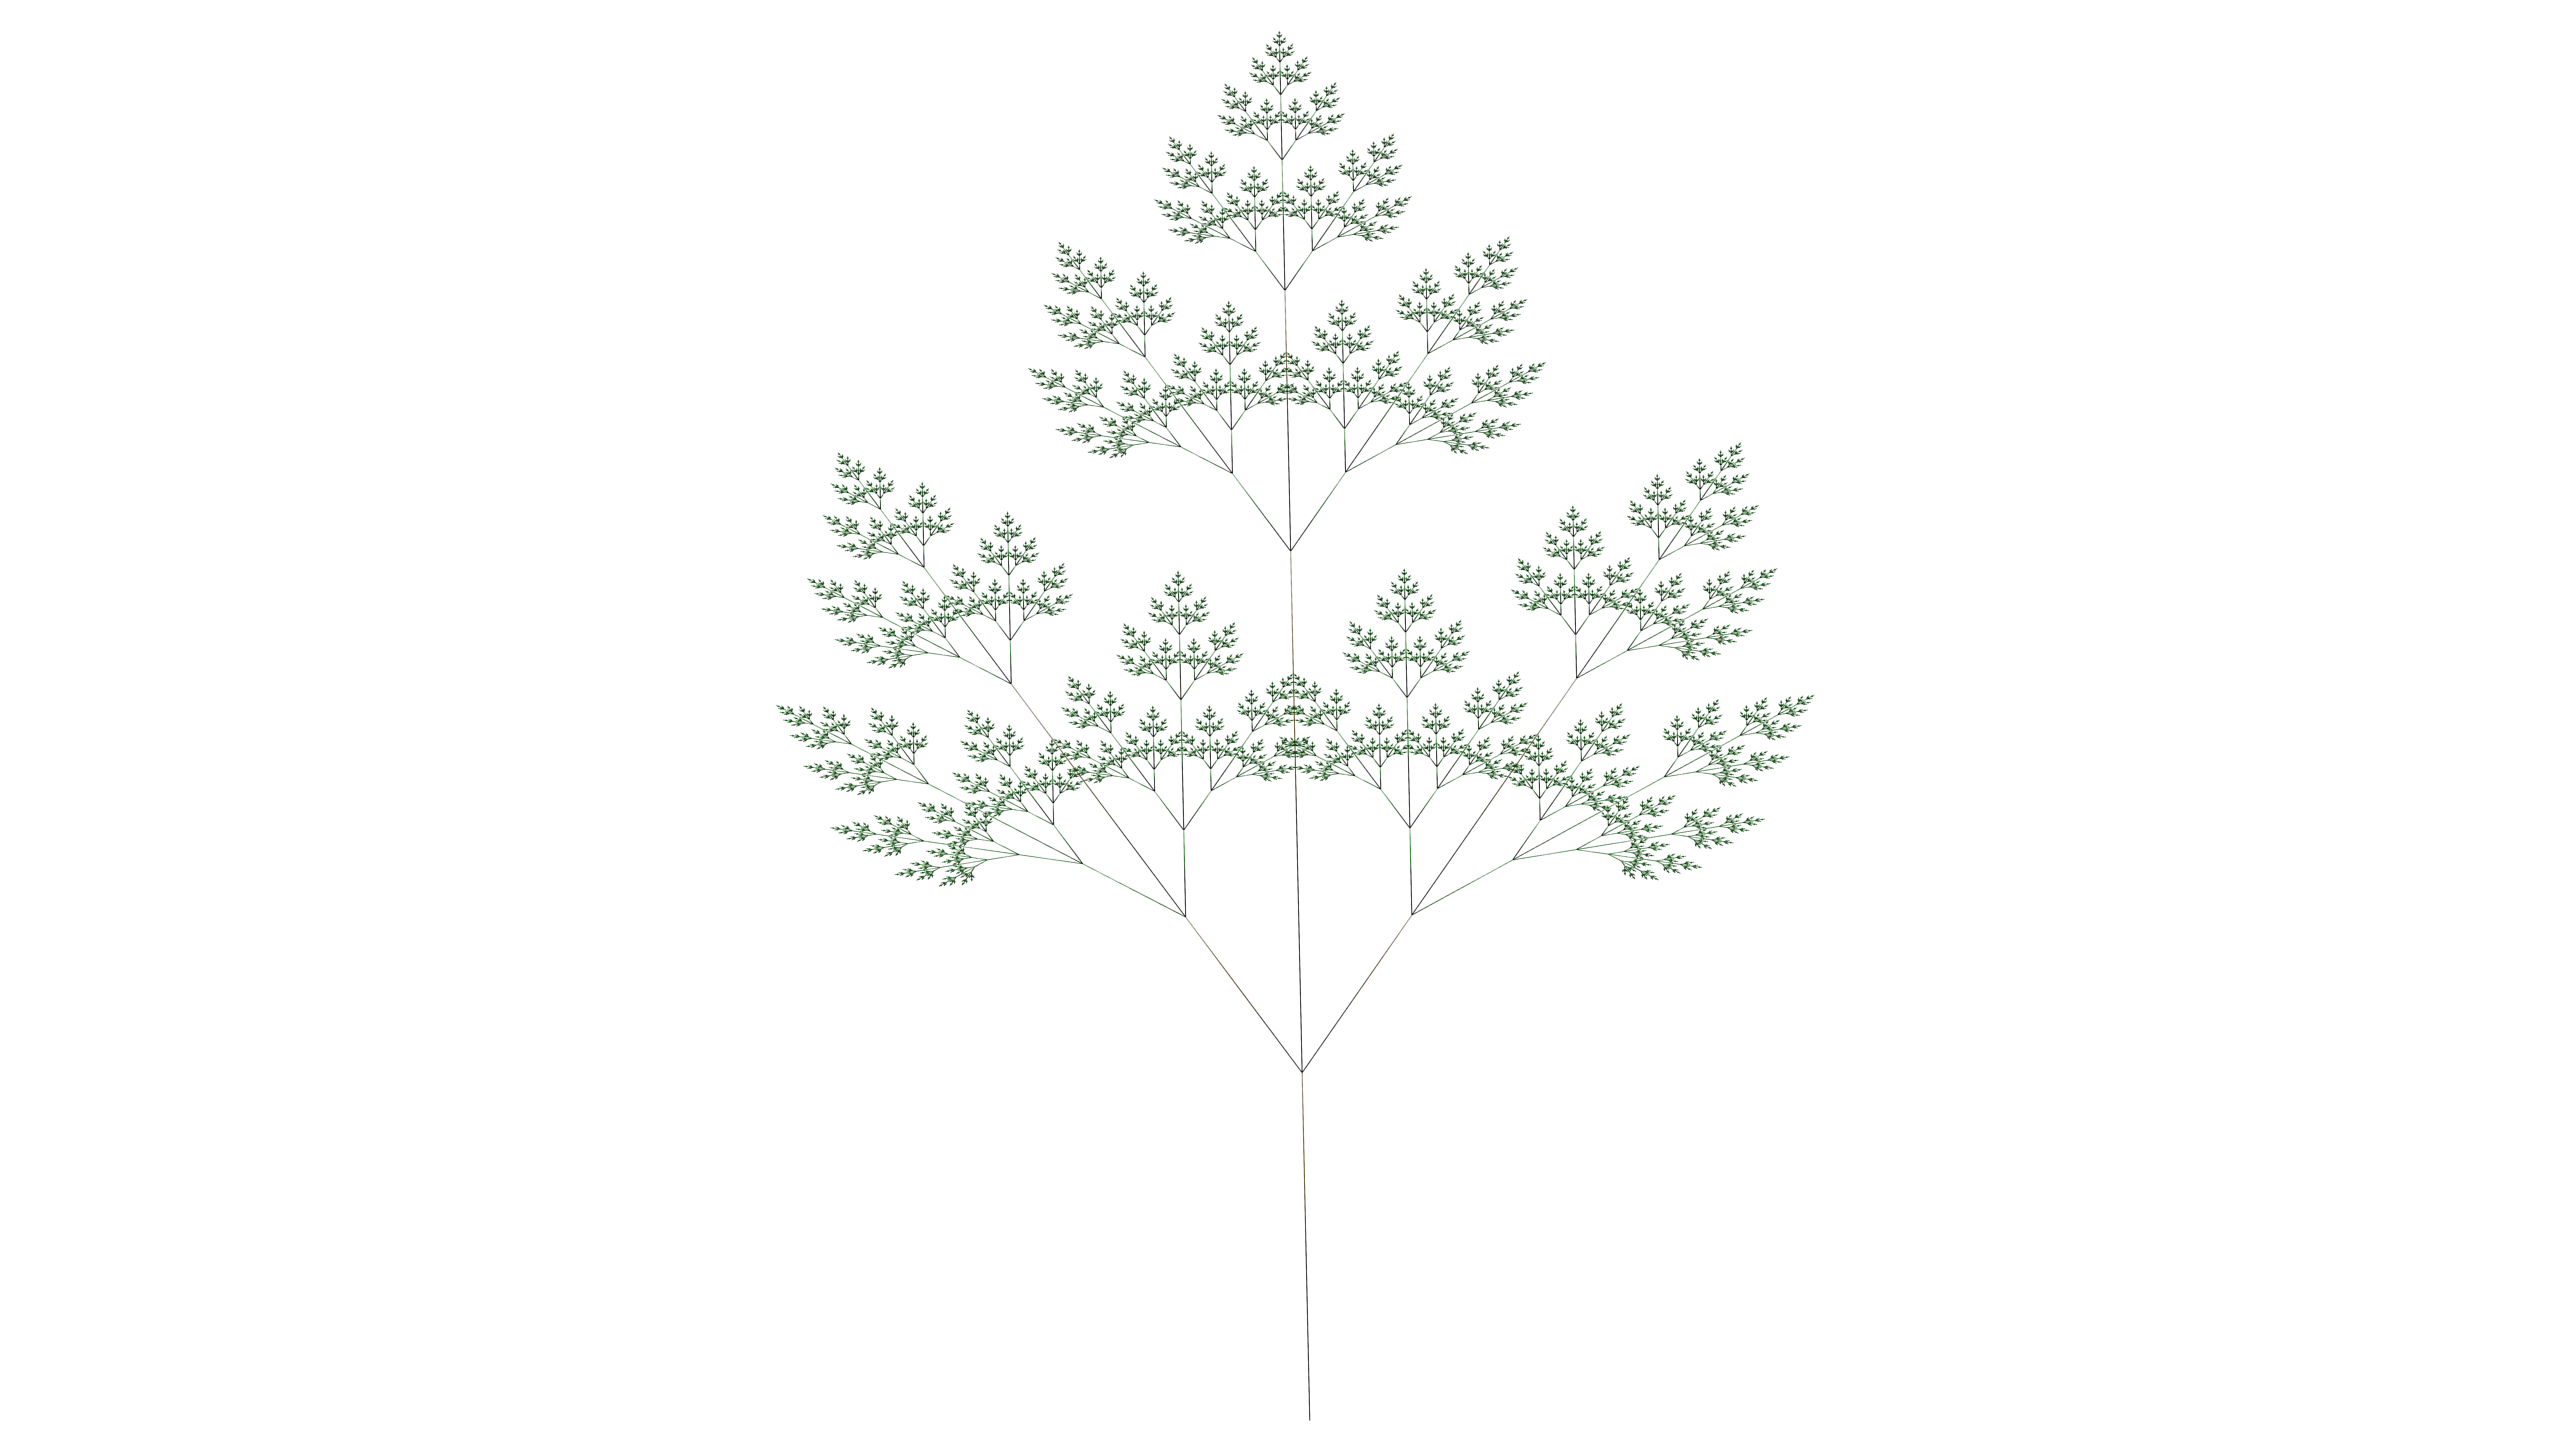
\includegraphics[width=0.90\textwidth]{figures/L-systems/e}
% \caption{Problem 2e}
% \label{fig:prob2e}
% \end{figure}

\begin{figure}[H]
\centering
\noindent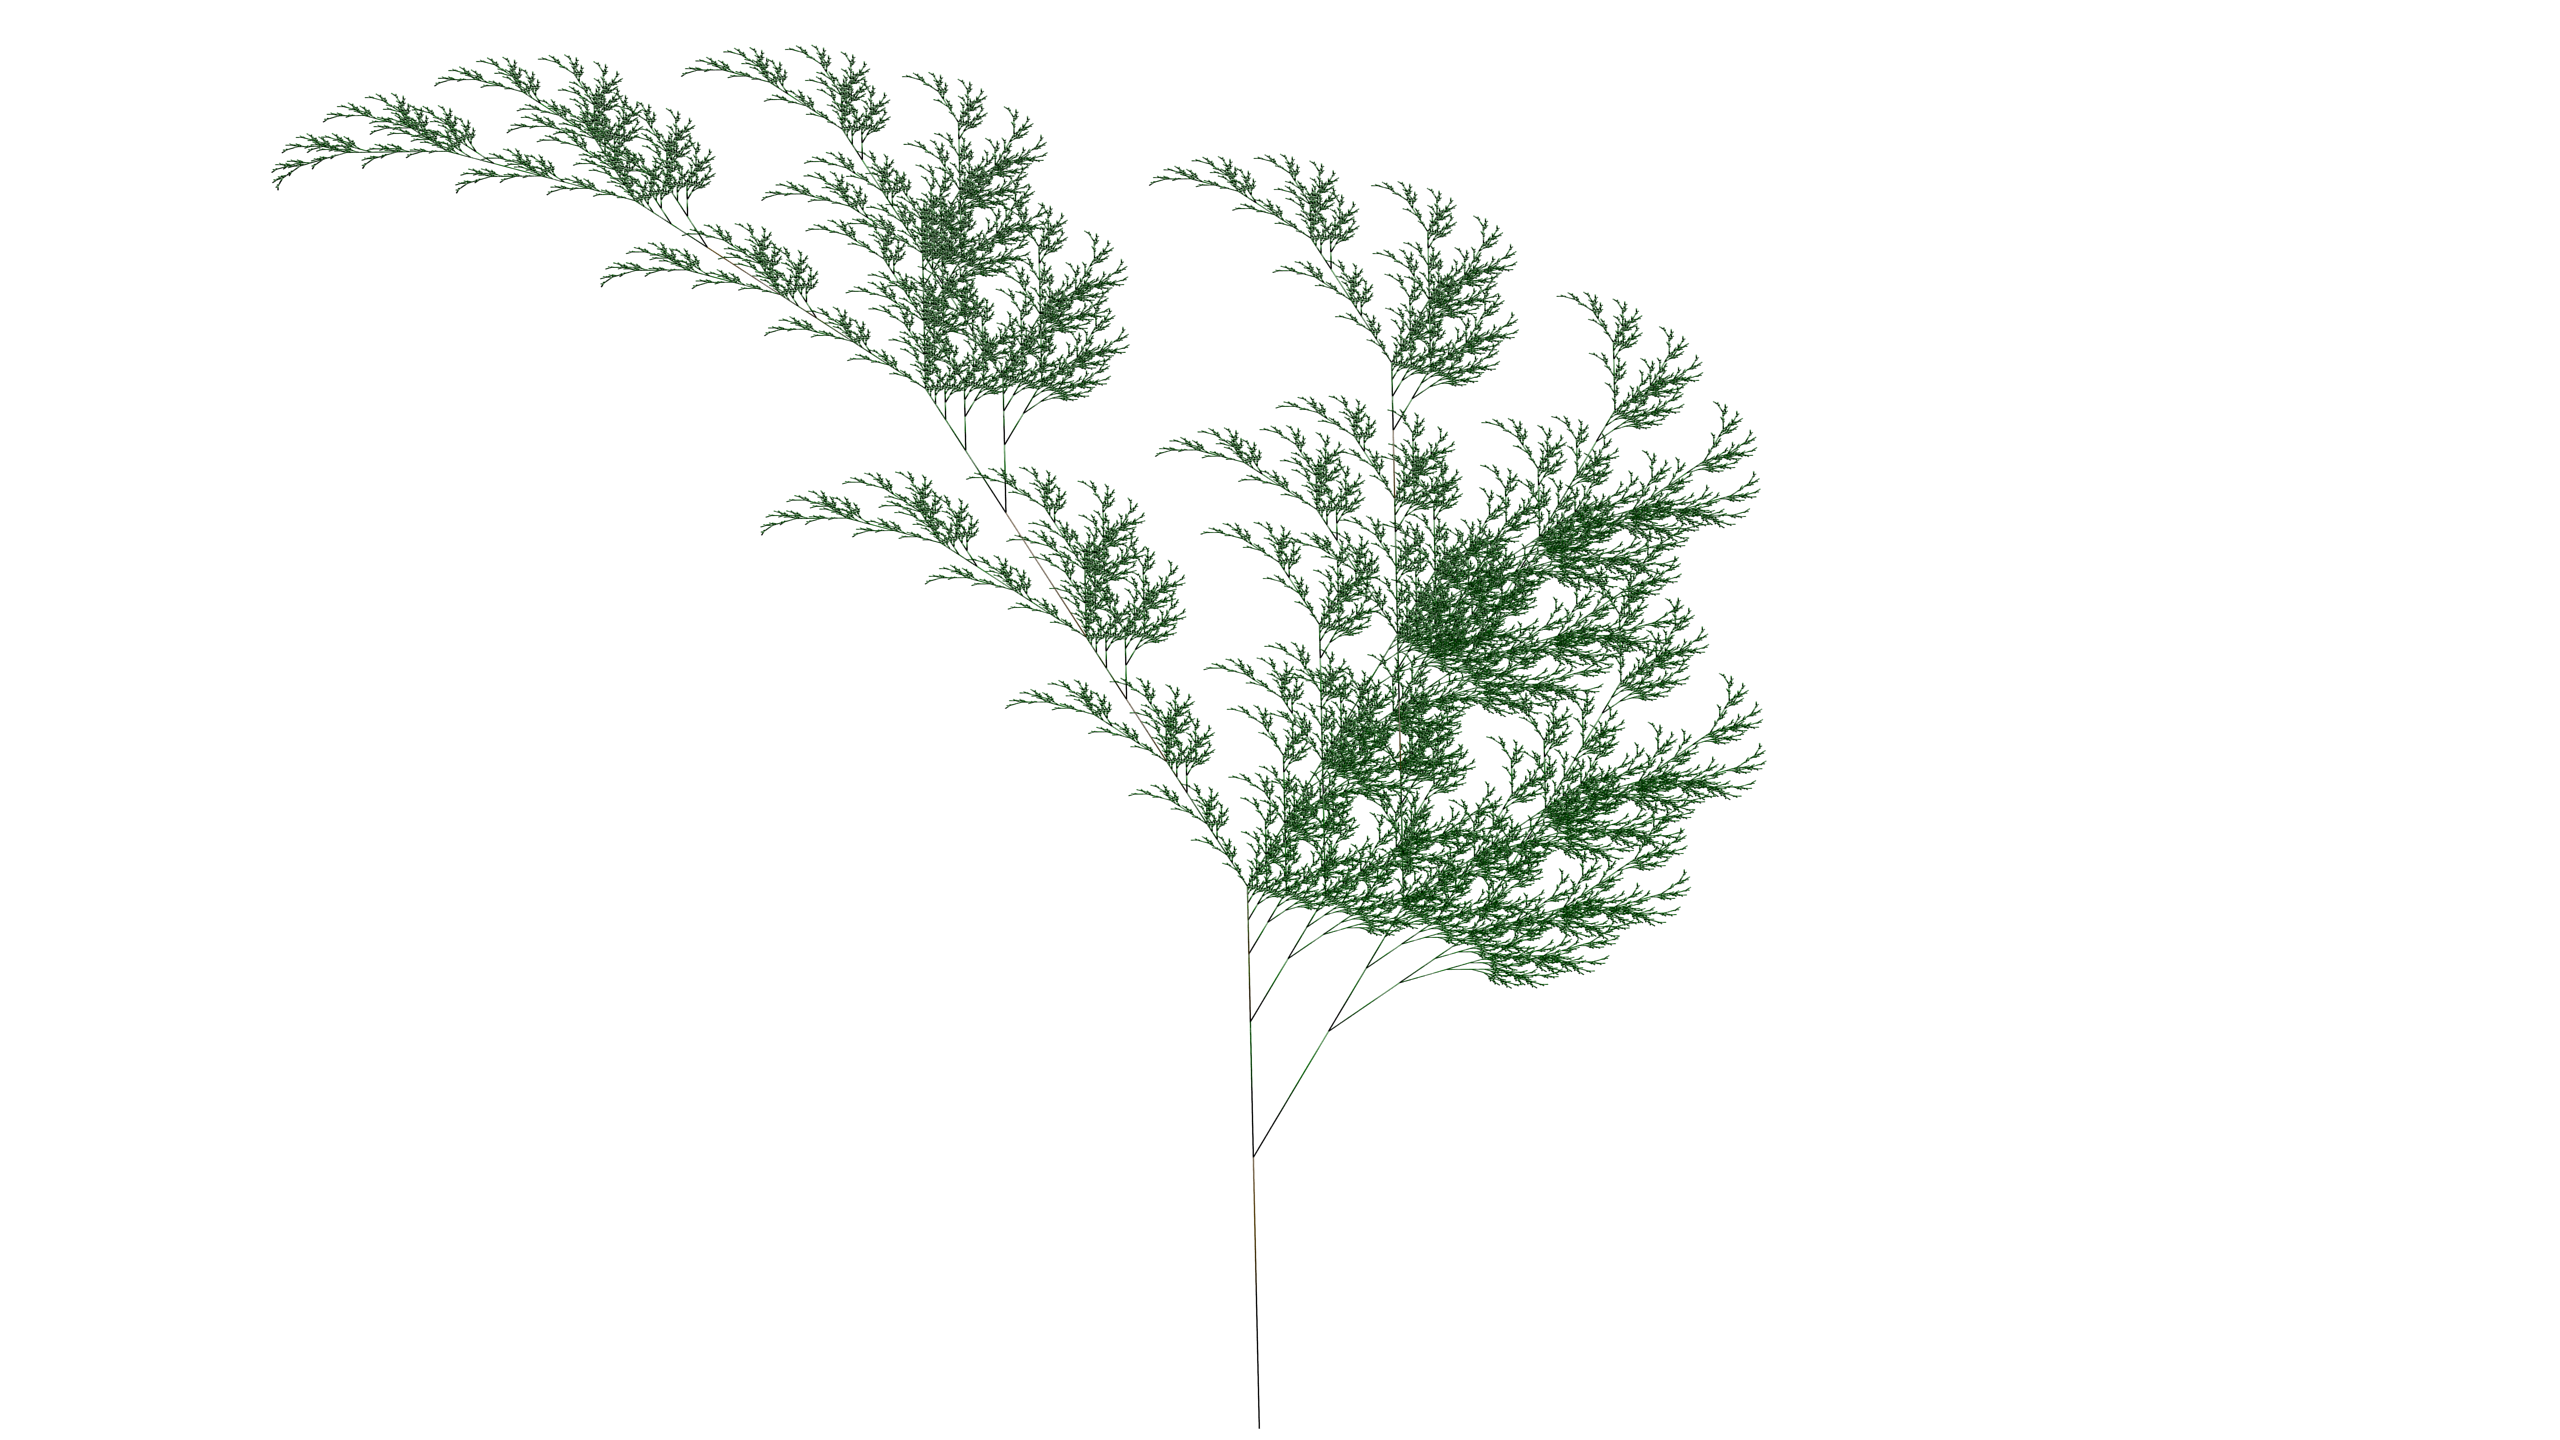
\includegraphics[width=0.90\textwidth]{figures/L-systems/a}
\caption{Problem 2a}
\label{fig:prob2a}
\end{figure}

\begin{figure}[H]
\centering
\noindent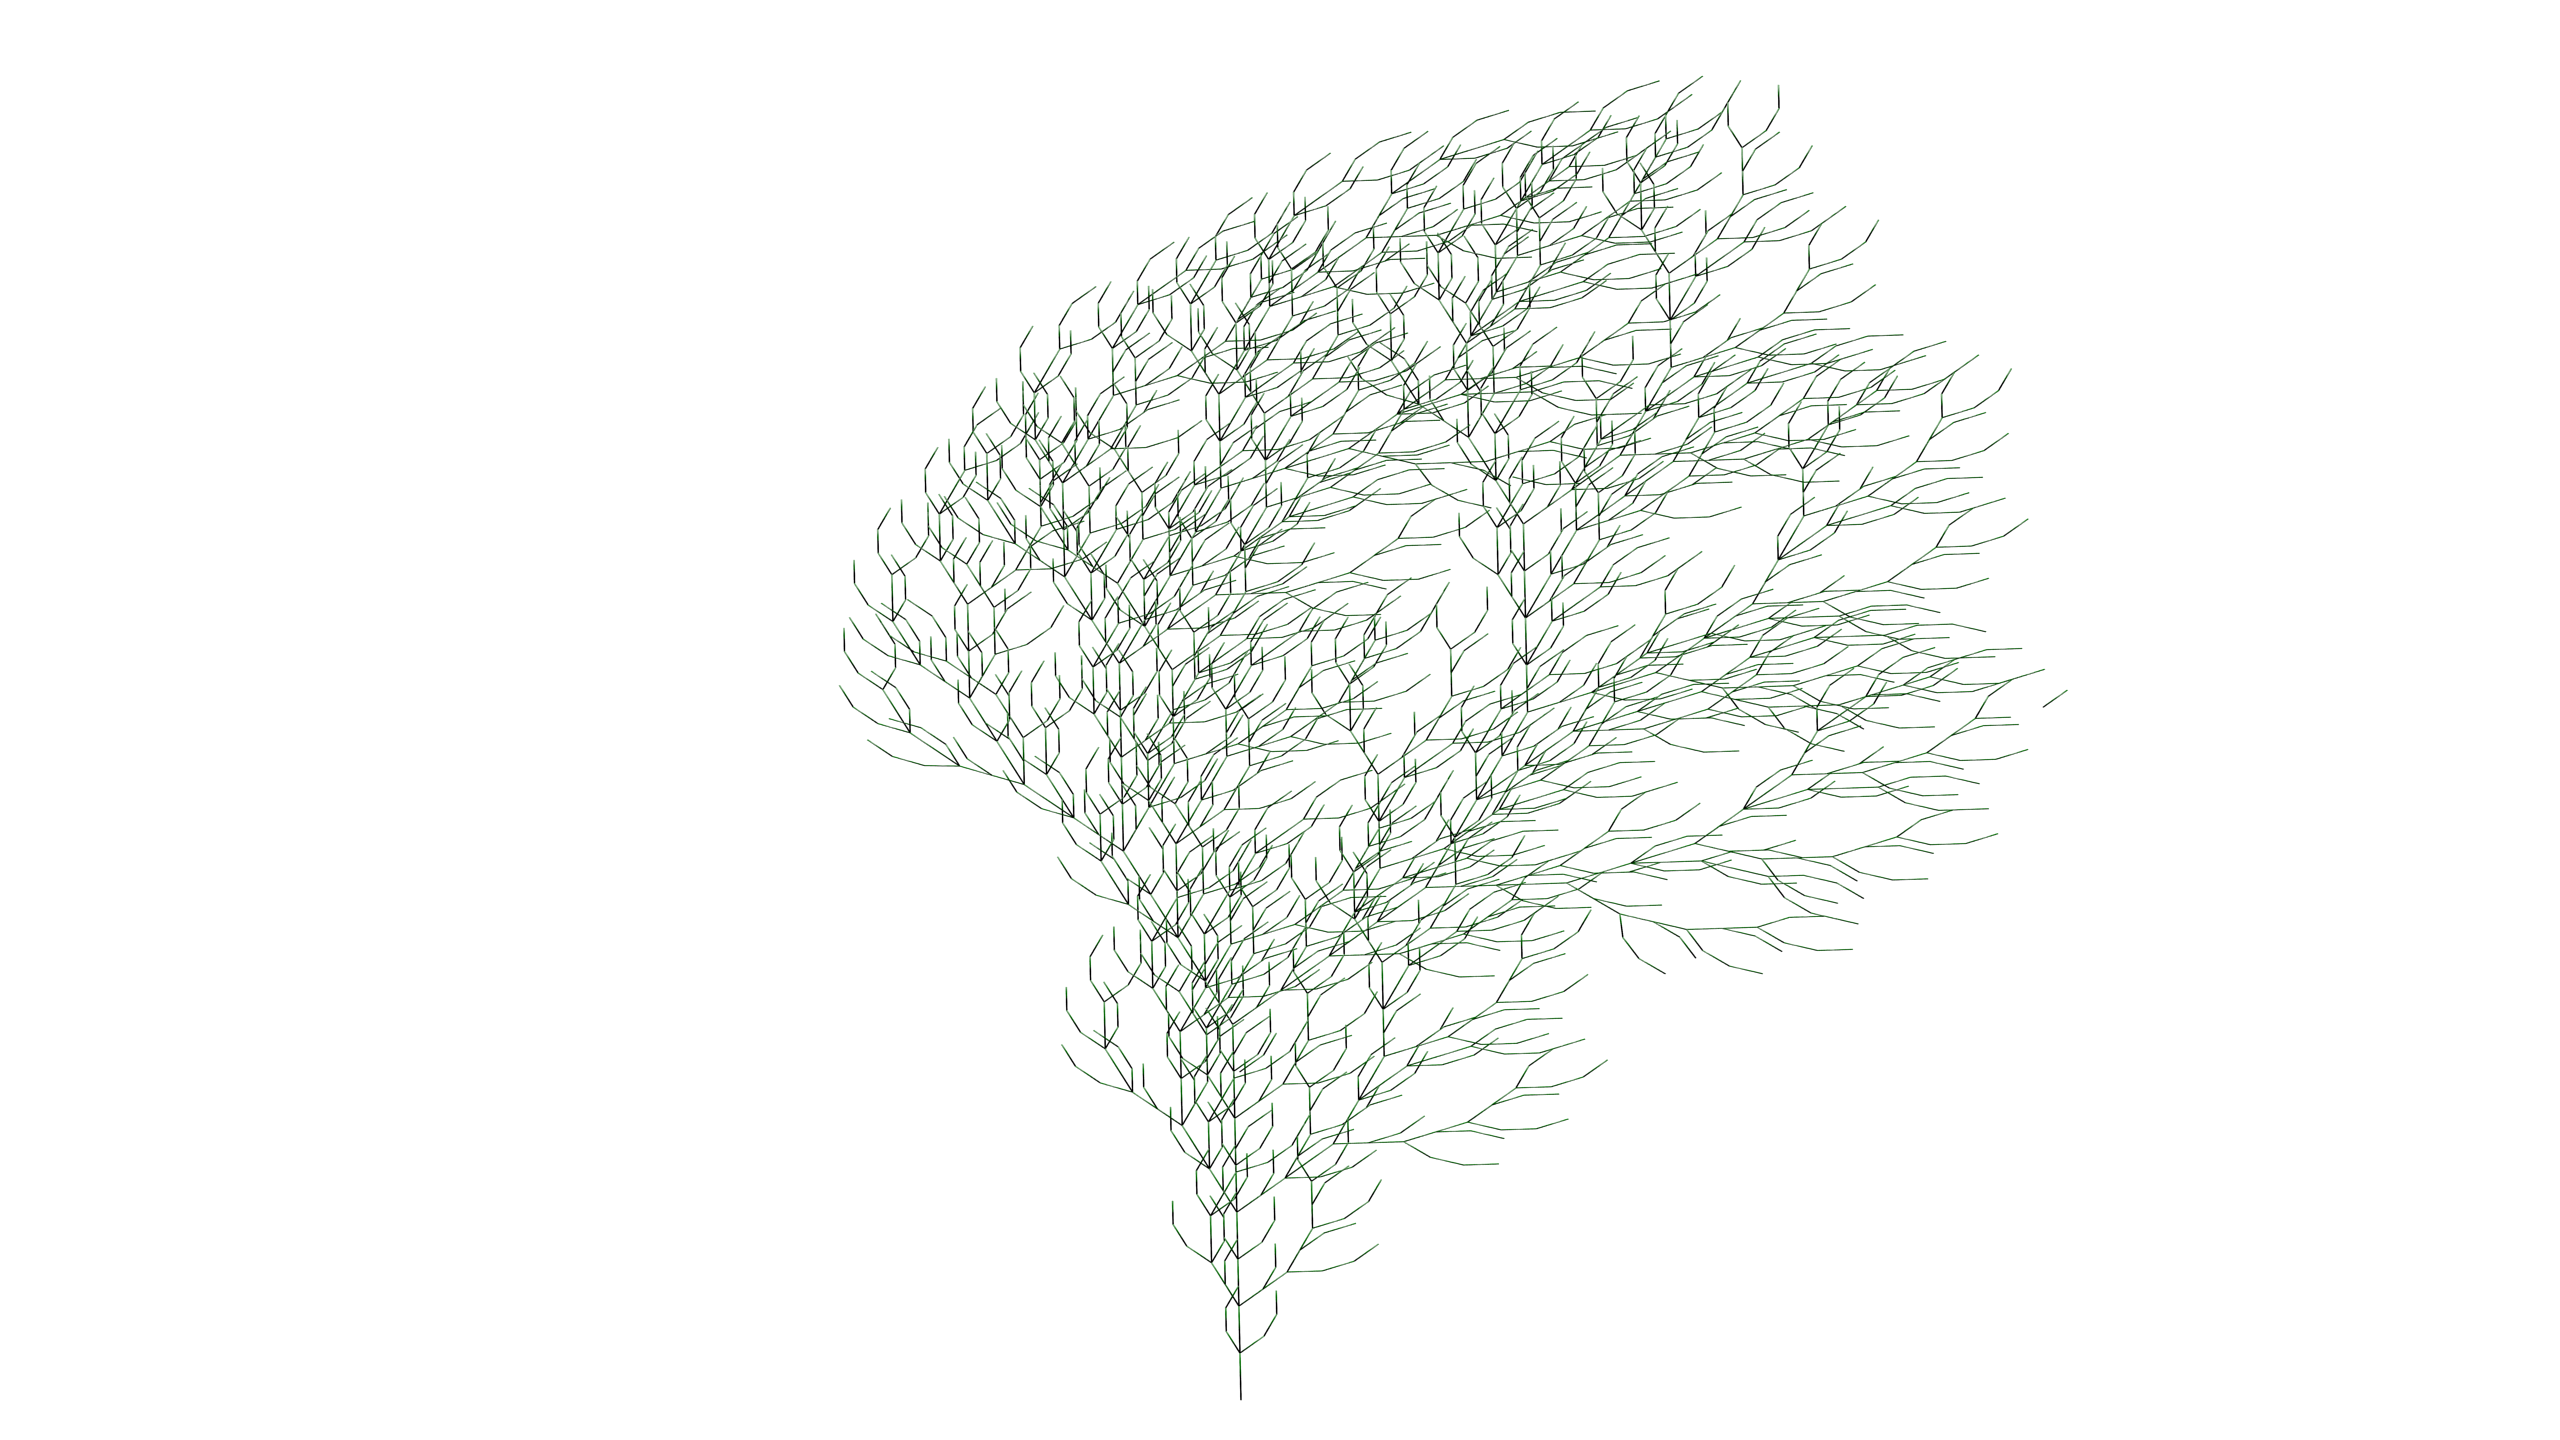
\includegraphics[width=0.90\textwidth]{figures/L-systems/b}
\caption{Problem 2b}
\label{fig:prob2b}
\end{figure}

\begin{figure}[H]
\centering
\noindent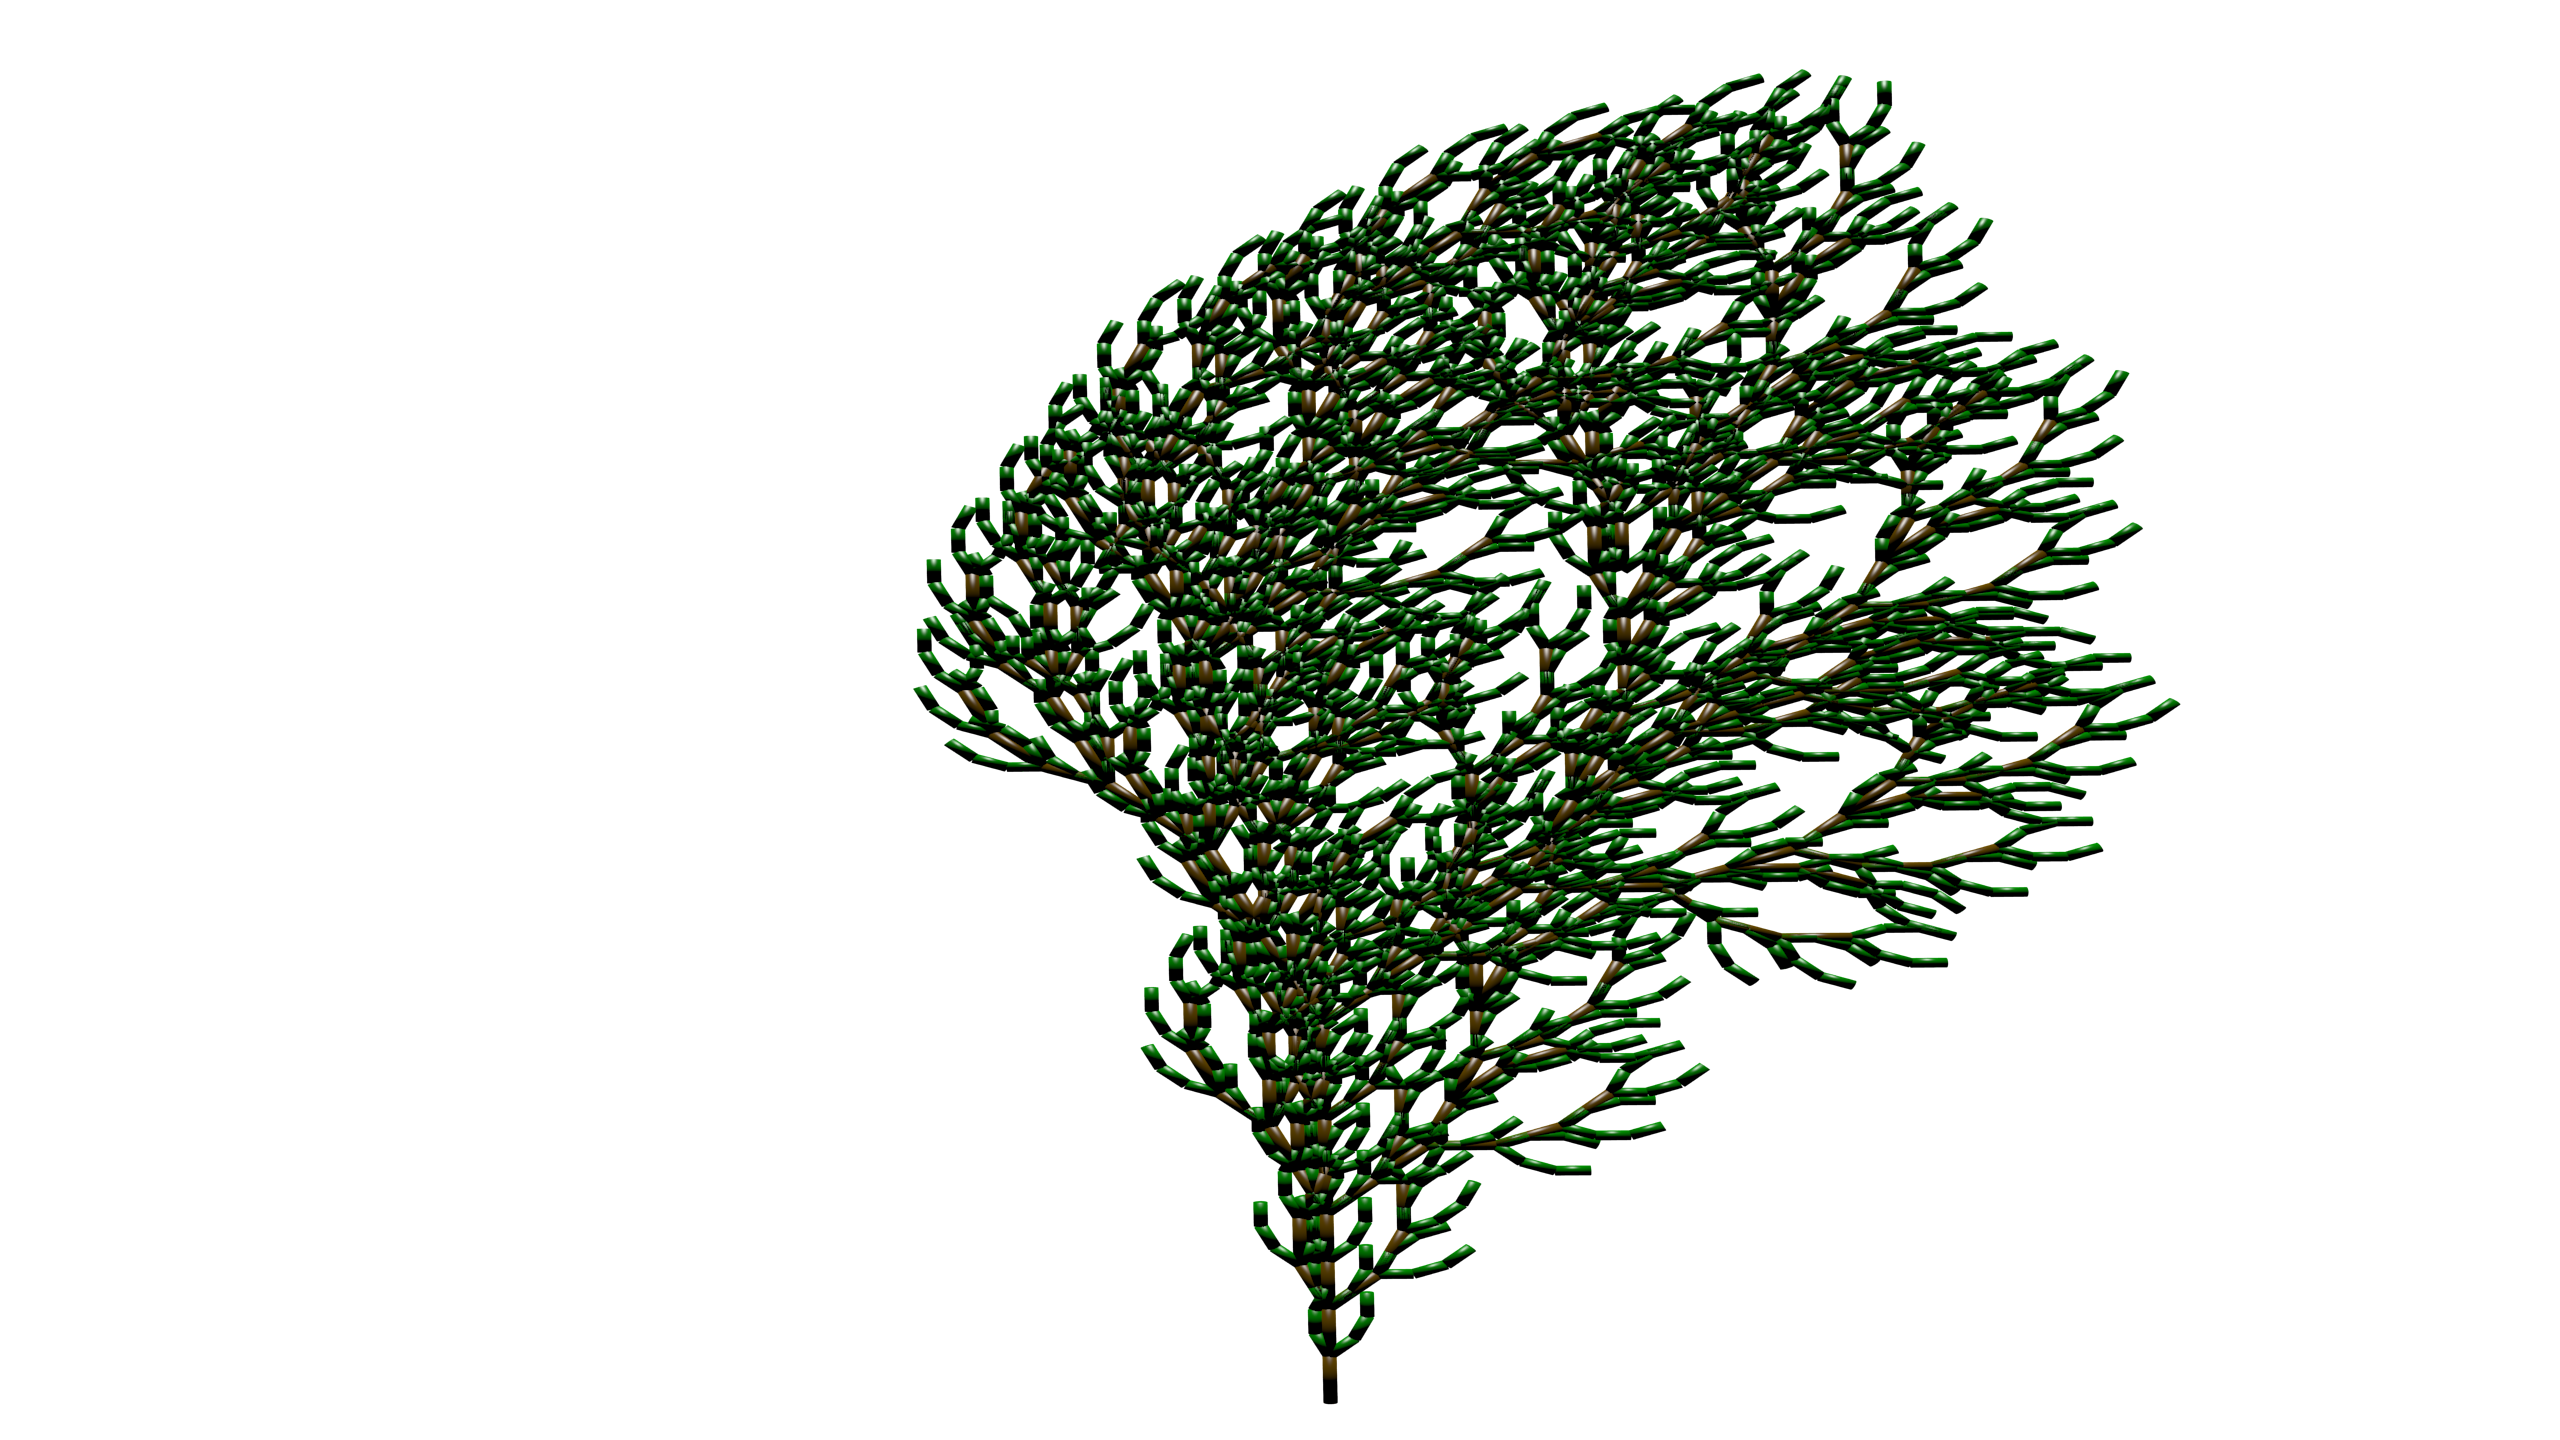
\includegraphics[width=0.90\textwidth]{figures/L-systems/b2}
\caption{Problem 2b2}
\label{fig:prob2b2}
\end{figure}

\begin{figure}[H]
\centering
\noindent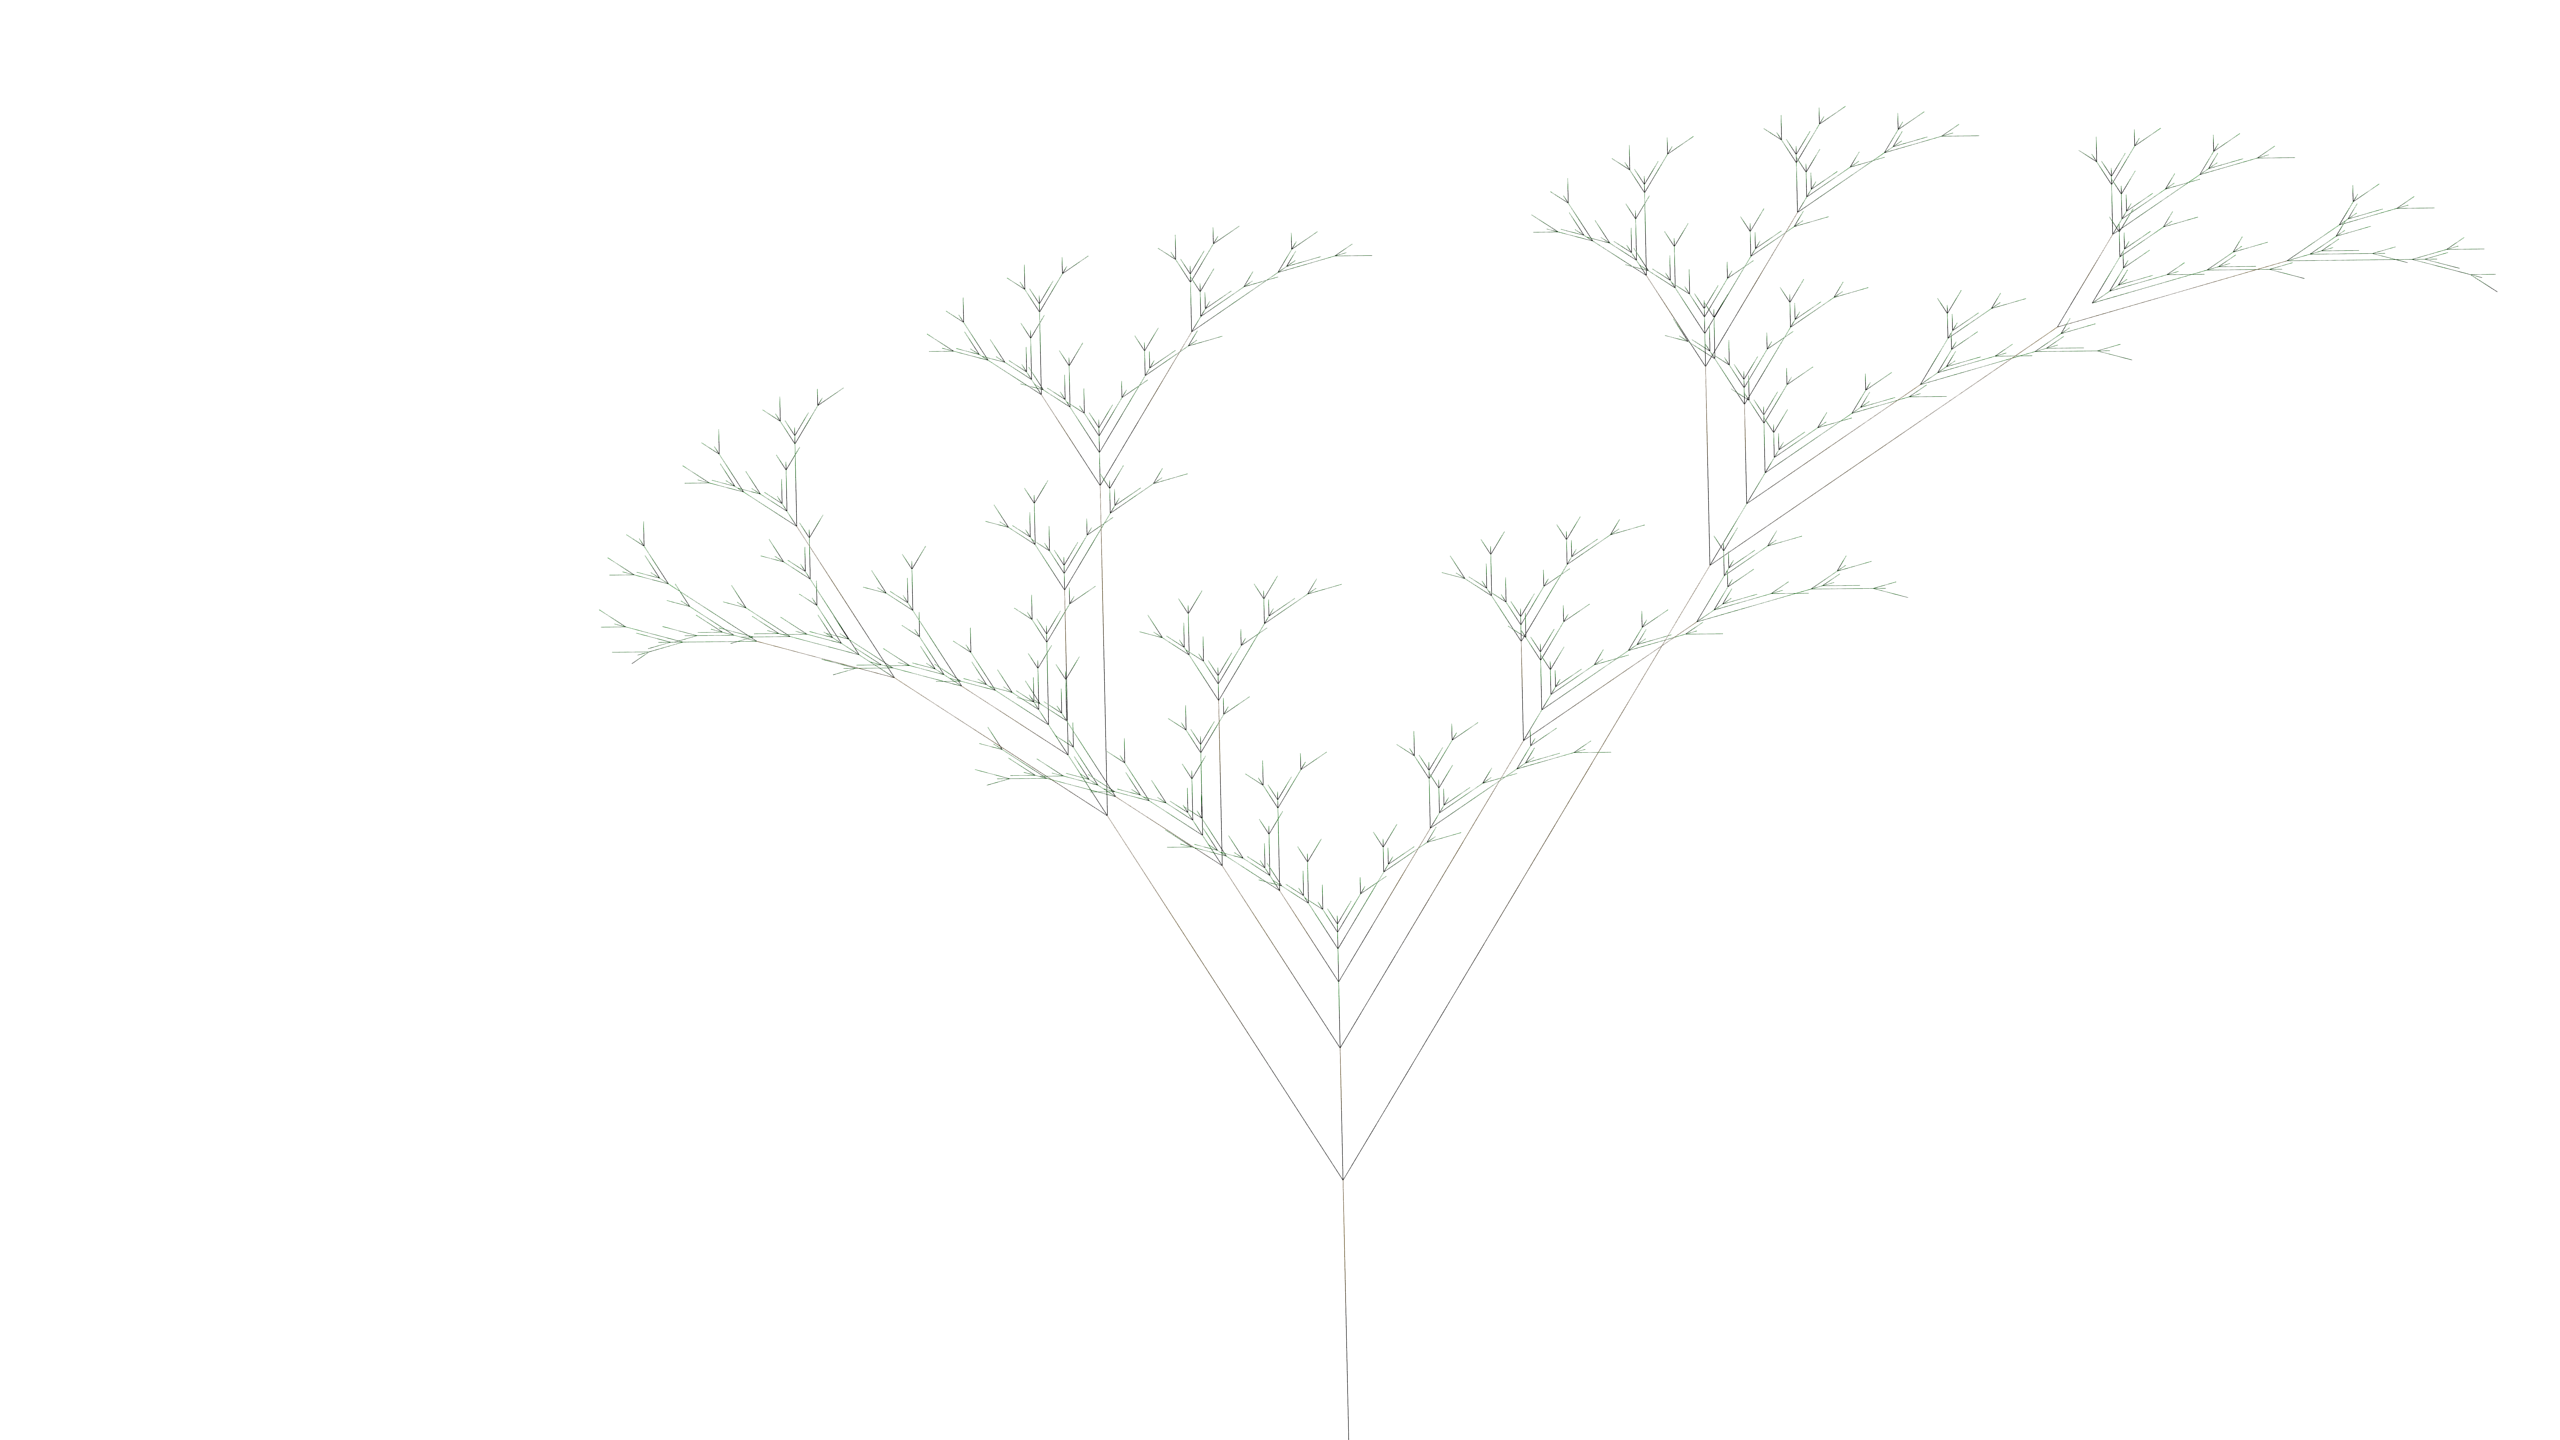
\includegraphics[width=0.90\textwidth]{figures/L-systems/c}
\caption{Problem 2c}
\label{fig:prob2c}
\end{figure}

\begin{figure}[H]
\centering
\noindent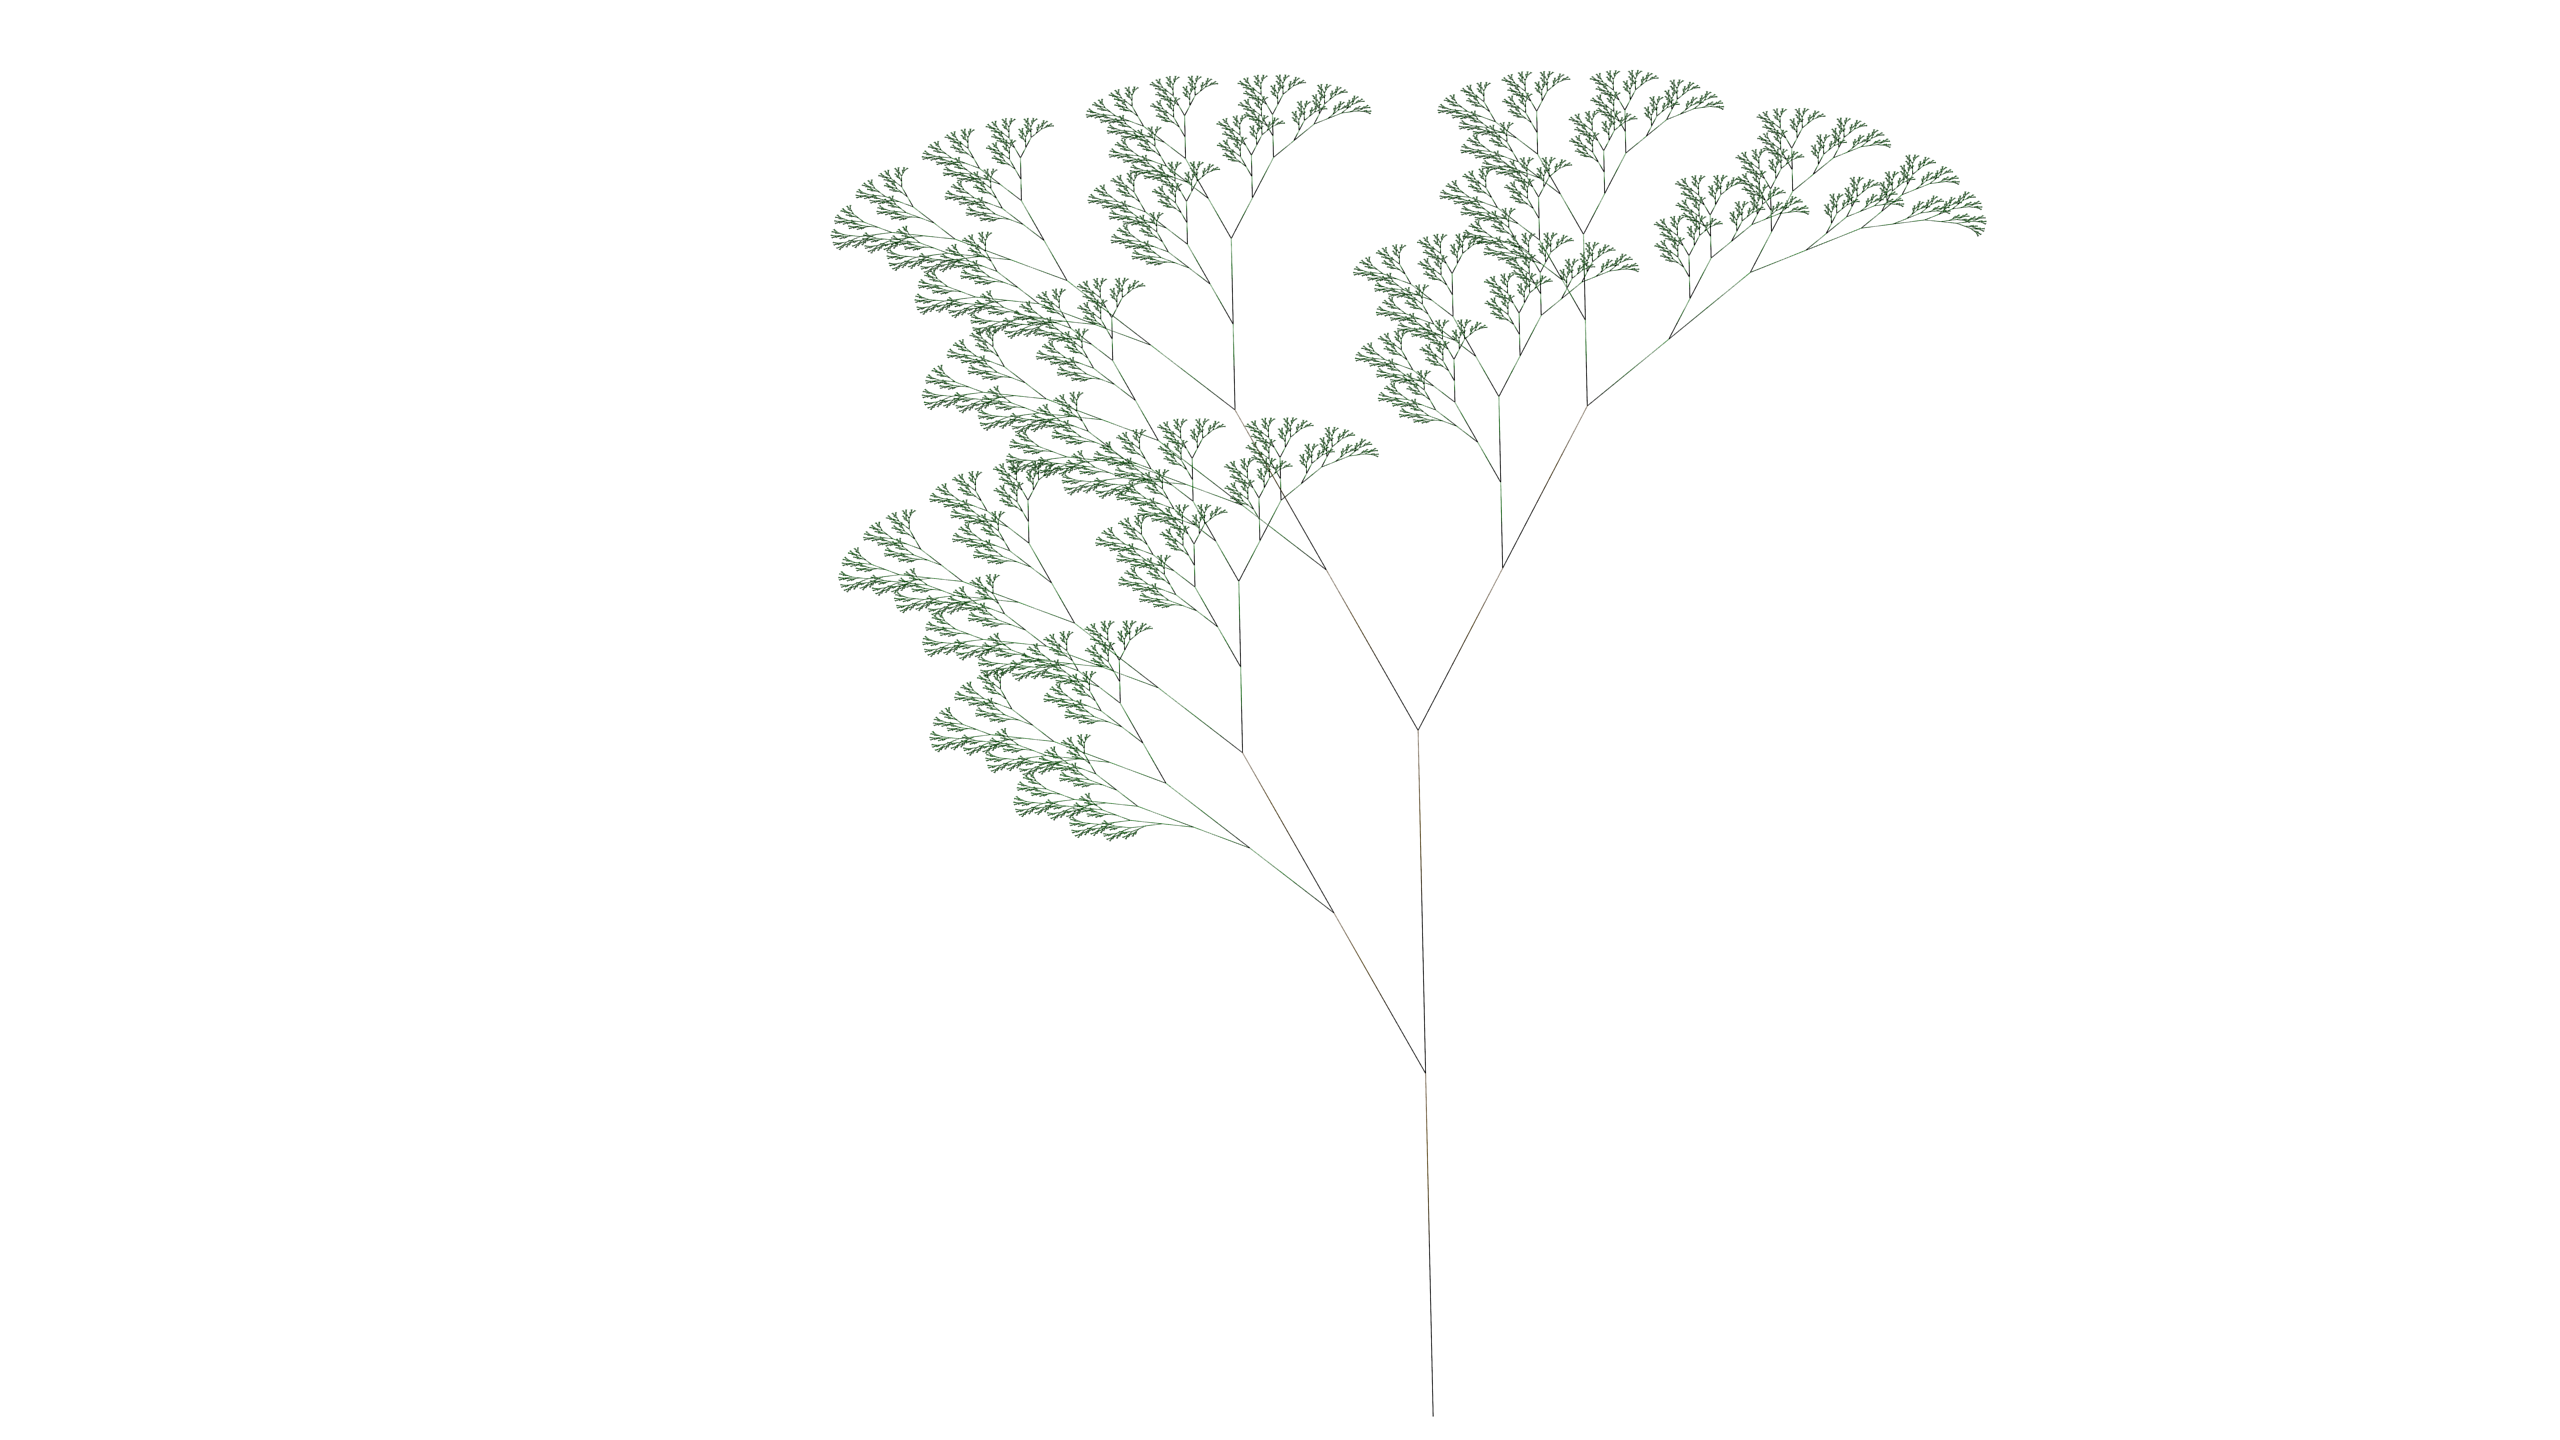
\includegraphics[width=0.90\textwidth]{figures/L-systems/d}
\caption{Problem 2d}
\label{fig:prob2d}
\end{figure}

\begin{figure}[H]
\centering
\noindent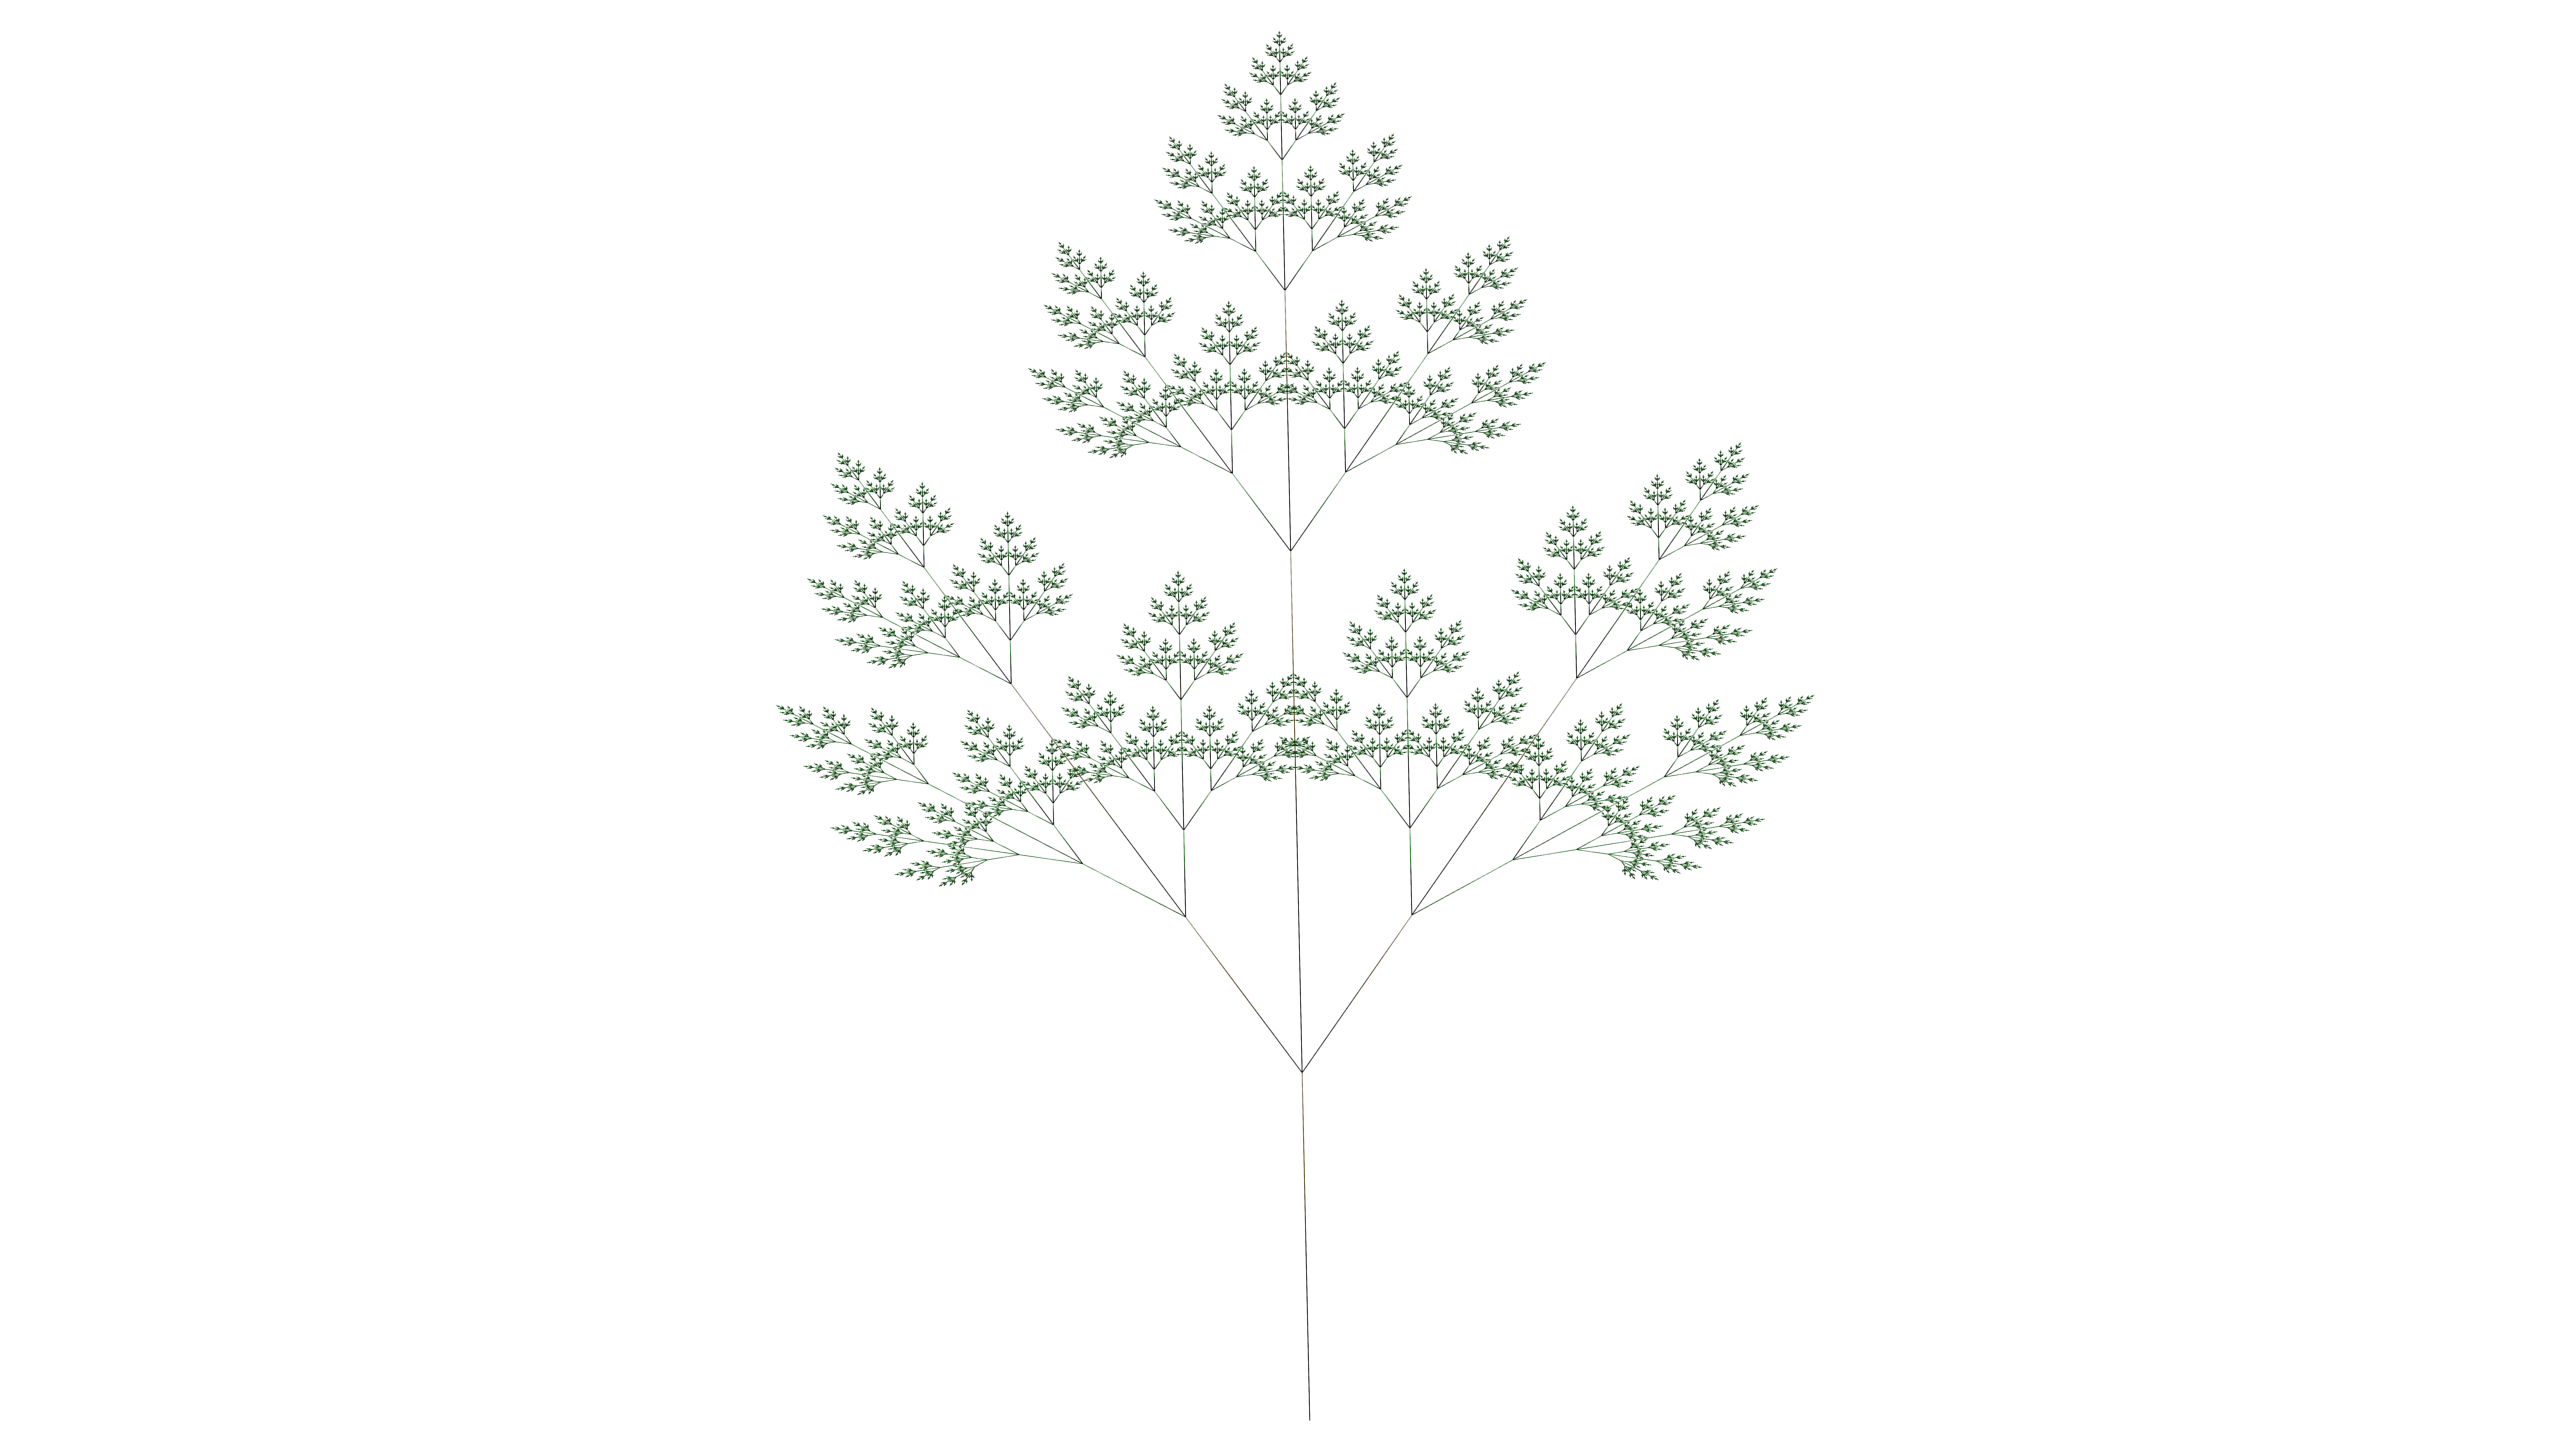
\includegraphics[width=0.90\textwidth]{figures/L-systems/e}
\caption{Problem 2e}
\label{fig:prob2e}
\end{figure}

\begin{figure}[H]
\centering
\noindent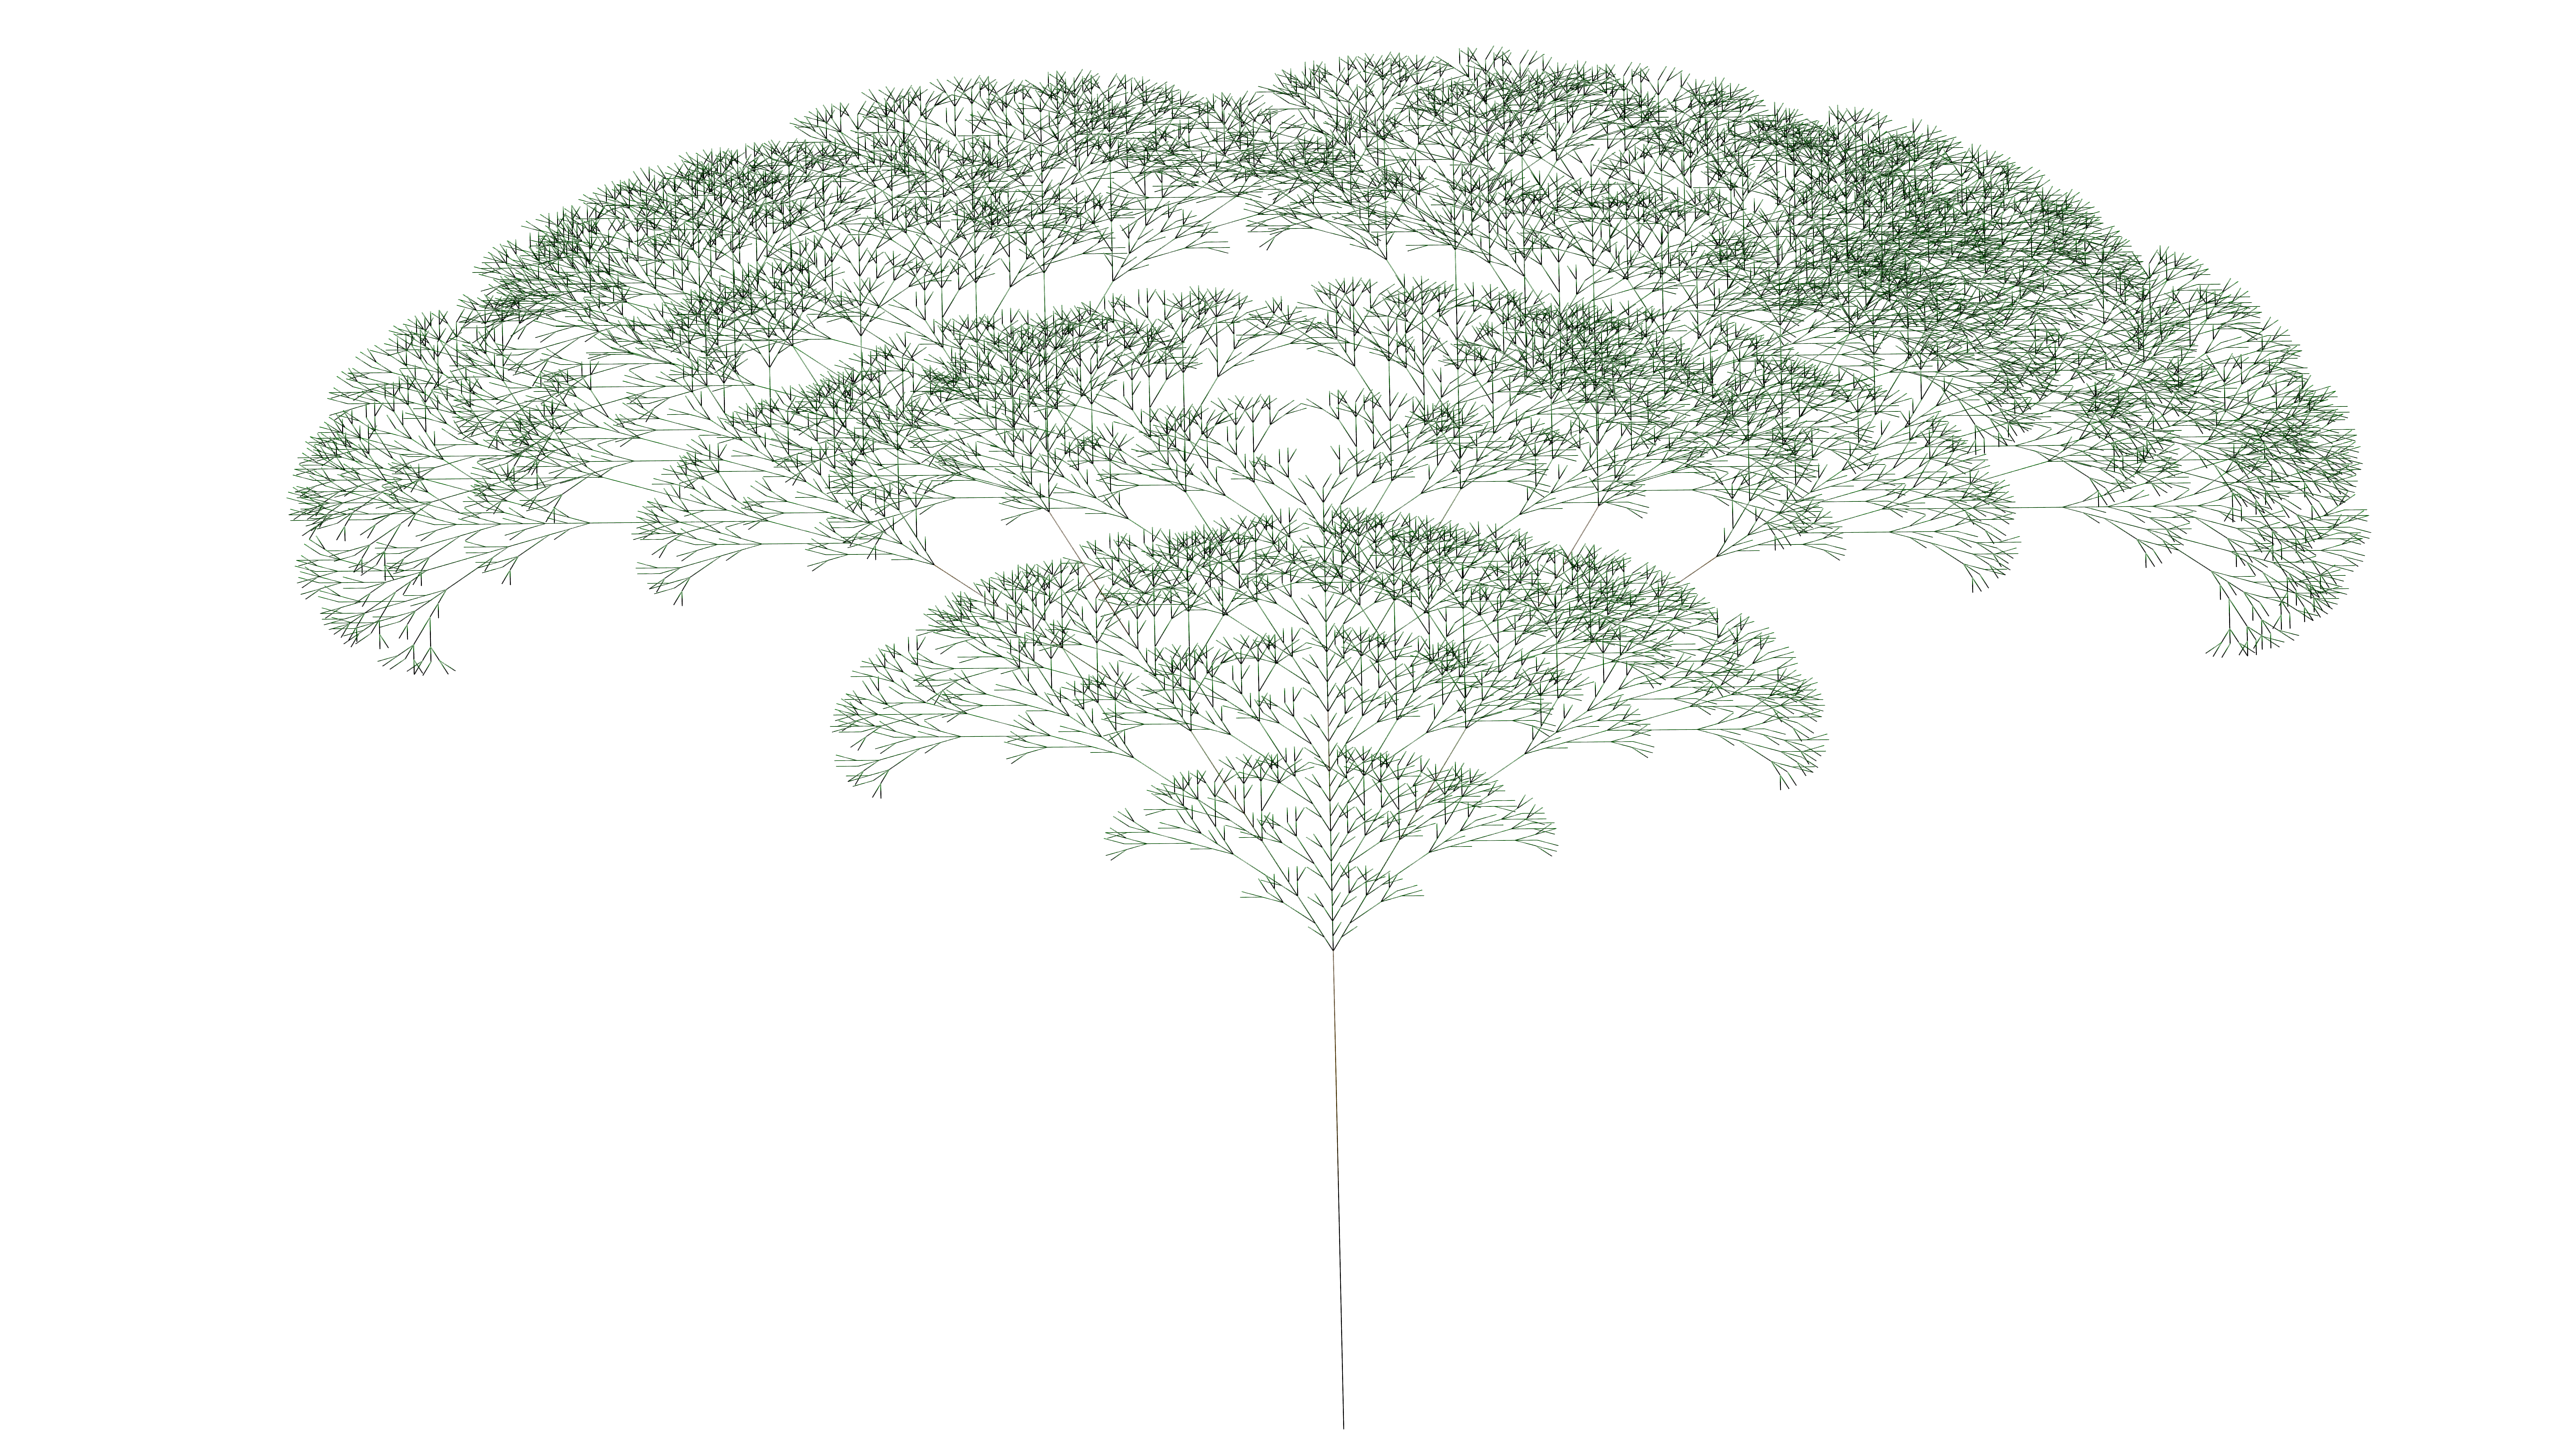
\includegraphics[width=0.90\textwidth]{figures/L-systems/f}
\caption{Problem 2f}
\label{fig:prob2f}
\end{figure}

\subsubsection{Expanding the Lindenmayer Systems to 3D}
\todoinline[caption=3d results]{
    Discuss how to create more interesting 3D fractals, including Koch curves, the dragon curve, and 3D trees/bushes.

    Show the results from \texttt{data/a.json} with the book's parameters.
}

\subsection{Conclusion}
